\documentclass[14pt]{beamer}
\usepackage[utf8]{inputenc}
\usepackage{polski}

\usetheme[height=1cm]{Rochester}
\usecolortheme[RGB={0,156,201}]{structure}
\usefonttheme{professionalfonts}
\setbeamertemplate{navigation symbols}{}

\title[Monady]{Monady, monady, monady}
\subtitle{Krótki wstęp}
\author{Łukasz Dąbek}

\begin{document}

\begin{frame}[plain]
    \titlepage
\end{frame}

\begin{frame}{Samouczki}
    \begin{center}
        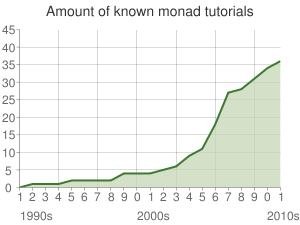
\includegraphics[scale=0.5]{monads-timeline.png}
    \end{center}
\end{frame}

\begin{frame}{Zwięzła definicja}
    \begin{quote}
        A monad is just a monoid in the category of endofuctors,
        what's the problem?
        \vskip5mm
        \hspace*\fill{\small--- Philip Wadler \pause (coż, nie do końca)} 
    \end{quote}
\end{frame}


\begin{frame}{I Ty możesz odkryć monady}
    \begin{itemize}
        \item Standardowa metoda: abstrakcyjne coś $\rightarrow$ zastosowania.
        \pause
        \item Dzisiejsza metoda: zastosowania $\rightarrow$ abstrakcyjne coś.
        \item (Podziękowania dla Dana Piponiego)
    \end{itemize}
\end{frame}

\begin{frame}{Funkcje debugowalne}
    \begin{itemize}
        \item Debugowanie w języku nieczystym jest proste
            (\texttt{printf} w dowolnym miejscu).
        \pause
        \item Jak poradzić sobie w Haskellu?
    \end{itemize}
\end{frame}

\begin{frame}{Funkcje debugowalne (2)}
    \texttt{f, g :: Float -> Float}
    \pause

    \texttt{f x = x * 4}

    \texttt{g x = x + 2}
\end{frame}

\begin{frame}{Funkcje debugowalne (2)}
    \texttt{f', g' :: Float -> (Float, \emph{String})}
    \pause

    \texttt{f' x = (x * 4, "f was called")}

    \texttt{g' x = (x + 2, "g " ++ show x)}
\end{frame}

\begin{frame}{Funkcje debugowalne - kompozycja}
    \begin{itemize}
        \item Chcemy prześledzić wykonanie złożenia funkcji \texttt{f'}
            i \texttt{g'}.
        \item Złożenie \texttt{f} i \texttt{g} to \texttt{f . g}.
        \item Jak złożyć \texttt{f'} i \texttt{g'}?
    \end{itemize}
\end{frame}

\begin{frame}[fragile]
\frametitle{Funkcje debugowalne - kompozycja}
\begin{verbatim}
let (y, s) = g' x
    (z, t) = f' y in (z, s ++ t)
\end{verbatim}
\end{frame}

\begin{frame}{Funkcje debugowalne - kompozycja}
    \begin{itemize}
        \item Nie chcemy pisać tego kodu wielokrotnie.
        \item \texttt{bind f' :: (Float,String) -> (Float,String)}
    \end{itemize}
\end{frame}

\begin{frame}[fragile]
\frametitle{Funkcje debugowalne - bind}
\begin{verbatim}
bind :: (Float -> (Float,String))
     -> (Float,String)
     -> (Float,String)
\end{verbatim}
\end{frame}

\begin{frame}[fragile]
\frametitle{Funkcje debugowalne - bind}
\begin{verbatim}
bind f (x,s) =
  let (y,t) = f x in (y,s ++ t)
\end{verbatim}
\end{frame}

\end{document}
